\maketitle

Due: Wednesday, March 13 at 11:59 pm. (Happy spring vacation!)

\section{Practice problems -- do not submit}
\subsection*{11.6. Gradients and directional derivatives}
\begin{practice}p.920 \#7\end{practice}
\begin{pracsol}
  \[\nabla f(x,y)=(f_x(x,y),f_y(x,y))=\left(\frac{y^2}{\cos(y)},\frac{xy(2\cos(y)+y\sin(y))}{\cos^2(y)}\right).\]
\end{pracsol}
\begin{practice}p.920 \#10\end{practice}
\begin{pracsol}
  \[\nabla f(x,y,z)=(y^2\sin(yz^2),2xy\sin(yz^2)+xy^2z^2\cos(yz^2),2xy^3z\cos(yz^2)).\]
\end{pracsol}
\begin{practice}p.920 \#13\end{practice}
\begin{pracsol}
  $\nabla f(x,y)=(-2x\sin(x^2-y^2),2y\sin(x^2-y^2))$. Therefore,
  \[D_\bu f\left(\sqrt\pi,\frac{\sqrt\pi}{2}\right)=\left(-\sqrt{2\pi},\frac{\sqrt{2\pi}}{2}\right)\cdot\left(\frac1{\sqrt2},-\frac1{\sqrt2}\right)=\frac{-3\sqrt{\pi}}{2}.\]
\end{pracsol}
\begin{practice}p.920 \#20\end{practice}
\begin{pracsol}
  \[\nabla f(x,y)=(ye^{xy}e^{-y},xe^{xy}e^{-y}-e^{xy}e^{-y}),\quad \nabla f(P_0)=(\ln(2),0),\quad D_\bu f(P_0)=0.\]
\end{pracsol}
\begin{practice}p.920 \#23\end{practice}
\begin{pracsol}
  \begin{enumerate}[(a)]
    \item $\bu$ is the unit vector having the same direction as
    \[\nabla f(P_0)=(3x^2y^2-y,2x^3y-x)\Big|_{(2,\frac12)}=\left(\frac52,6\right).\]
    \item $D_\bu(f)(P_0)=\|\nabla f(P_0)\|=\frac{13}2$.
    \item $\bv=-\bu=-\left(\frac5{13},\frac{12}{13}\right)$.
    \item $D_\bv f(P_0)=-\frac{13}2$.
  \end{enumerate}
\end{pracsol}
\begin{practice}p.920 \#35\end{practice}
\begin{pracsol}
  Since $\nabla F(x,y,z)=(yz\cos(xz),\sin(xz),xy\cos(xz))$,
  \[D_\bu F\left(\frac12,3,\pi\right)=(0,1,0)\cdot\left(\frac{\sqrt3}{8},-\frac68,\frac58\right)=-\frac34.\]
\end{pracsol}
\begin{practice}p.920 \#39\end{practice}
\begin{pracsol}
  Since $\nabla F(x,y,z)=(2x(y^3-yz),x^2(3y^2-z),-x^2)$,
  \begin{enumerate}[(a)]
    \item $\bu$ is the unit vector having the same direction as
    \[\nabla F(2,1,4)=(12,-4,4)=4(3,-1,1).\]
    \item $D_\bu F(P_0)=\|\nabla f(P_0)\|=4\sqrt{11}$.
    \item $\bv=-\frac1{\sqrt{11}}(3,-1,1)$.
    \item $D_\bv F(P_0)=-4\sqrt{11}$.
  \end{enumerate}
\end{pracsol}
\begin{practice}p.921 \#44\end{practice}
\begin{pracsol}
  We calculate $\bu=\|\overrightarrow{PQ}\|^{-1}\overrightarrow{PQ}=\left(\frac1{\sqrt2},\frac1{\sqrt2}\right)$, $\nabla f(x,y)=(2x+y+x)$, $\nabla f(P)=(4,1)$, and $D_\bu f(P)=(4,1)\cdot\left(\frac1{\sqrt2},\frac1{\sqrt2}\right)=5\sqrt2$.
\end{pracsol}
\begin{practice}p.921 \#48\end{practice}
\begin{pracsol}
  Let $\nabla f(P)=(s,t)$. We are given t he equations $0s+1t=2\sqrt2$ and $\frac1{\sqrt2}s+\frac1{\sqrt2}t=3\sqrt2$. The first equation gives us $t=2\sqrt2$, and when we substitute this value into the second equation, we obtain $s=6-2\sqrt2$. Thus $f_x(P)=6-2\sqrt2$ and $f_y(P)=2\sqrt2$.
\end{pracsol}
\begin{practice}p.921 \#55\end{practice}
\begin{pracsol}
  The missile will move in the direction of the gradient, $\nabla T(100,15,8)$. Since $\nabla T(x,y,z)=(-20(x-90),-8(y-12)^3,-2z)$,
  \[\nabla T(100,15,8)=-(200,216,16)=-8(25,27,2).\]
  Therefore, the direction is
  \[\bu=-\frac1{\sqrt{1358}}(25,27,2).\]
\end{pracsol}

\subsection*{11.7. Tangent planes}
\begin{practice}p.931 \#1\end{practice}
\begin{pracsol}
  Since $\nabla f(x,y)=(y+2x,x-3y^2)$, $\nabla f(1,4)=(6,-47)$. Therefore, the vector $\mathbf N=(6,-47,-1)$ is normal to the plane and, since $f(1,4)=-59$, its equation is $6(x-1)-47(y-4)-(z+59)=0$ or $z=6x-47y+123$.
\end{pracsol}
\begin{practice}p.931 \#2\end{practice}
\begin{pracsol}
  We calculate $\nabla f(x,y)=(\cos(x-y),-\cos(x-y))$ and $\nabla f(P_0)=\left(\frac{\sqrt3}2,-\frac{\sqrt3}2\right)$. A normal vector is $\left(\frac{\sqrt3}2,-\frac{\sqrt3}2,-1\right)$ and the equation of the tangent plane is
  \[z=\frac{\sqrt3}2\left(x-\frac{\pi}2\right)-\frac{\sqrt3}2\left(y-\frac{\pi}2\right)+\frac12.\]
\end{pracsol}
\begin{practice}p.931 \#4\end{practice}
\begin{pracsol}
  We calculate $\nabla f(x,y)=(2e^{2x-3y},-3e^{2x-3y})$ and $\nabla f(P_0)=\left(\frac8{27},-\frac49\right)$. A normal vector is $\left(\frac8{27},-\frac49,-1\right)$ and the equation of the tangent plane is
  \[z=\frac8{27}(x-\ln(2))-\frac49(y-\ln(3))+\frac4{27}.\]
\end{pracsol}
\begin{practice}p.931 \#14\end{practice}
\begin{pracsol}
  Letting $F(x,y,z)$ be the left side of the equation, we calculate $\nabla F(x,y,z)=(yz,xz,xy)$ and $\nabla F(Q_0)=(2,8,4)$, which is a normal vector to the surface at $Q_0$. The equation of the tangent plane is
  \[2x+8y+4z=24.\]
\end{pracsol}
\begin{practice}p.931 \#20\end{practice}
\begin{pracsol}
  Letting $F(x,y,z)$ be the left side of the equation, we calculate
  \[\nabla F(x,y,z)=(-yz\sin(xyz),-xz\sin(xyz),-xy\sin(xyz))\]
  and $\nabla F(Q_0)=\left(-\frac{\pi}8,-\frac12,-4\pi\right)$ which is a normal vector to the surface at $Q_0$. The equation of the tangent plane is
  \[-\frac{\pi}8(x-4)-\frac12(y-\pi)-4\pi\left(z-\frac18\right)=0.\]
  If you want, you can multiply both sides by $-8$ to obtain the simpler equation
  \[\pi(x-4)+4(y-\pi)+4\pi\left(8z-1\right)=0.\]
\end{pracsol}

\newpage

\section{Homework problems -- submit these}
\begin{problem}\leavevmode
  \begin{enumerate}[(a)]
    \item A rectangular box has sides that, due to temperature fluctuations, undergo changes in dimension. At a given moment, the length increases at a rate of 0.01 cm/s, the width decreases at a rate of 0.02 cm/s, and the height increases at a rate of 0.005 cm/s. At this particular moment, the length is 15 cm, the width is 8 cm, and the height is 5 cm. Is the volume increasing or decreasing at this moment?
    \begin{solution}
      There are two main solutions, the first using the multivariable chain rule and the second using the product rule.

      Volume is $V=\ell w h$, where $\ell,w,h$ are length, width, and height respectively. So we may write $V$ as a 3-variable function
      \[V(\ell,w,h)=\ell w h.\]
      Here, each of $\ell,w,h$ are functions of $t$, so we can express the volume at time $t$ as $V(\ell(t),w(t),h(t))$. Let $t_0$ be the current moment in time. We are given:
      \begin{align*}
        \ell(t_0) &= 15,&w(t_0)&=8,&h(t_0)&=5,\\
        \ell'(t_0) &= 0.01,&w'(t_0)&=-0.02,&h'(t_0)&=0.005.
      \end{align*}
      If we use the multivariable chain rule, we find
      \[\begin{split}
        \frac d{dt}\Big|_{t=t_0}V(\ell(t),w(t),h(t)) &= \frac{\partial V}{\partial\ell}\ell'(t_0)+\frac{\partial V}{\partial w}w'(t_0)+\frac{\partial V}{\partial h}h'(t_0)\\
        & \begin{multlined}= (w(t_0)h(t_0))(0.01)+(\ell(t_0) h(t_0))(-0.02)+\\
          \ell(t_0) w(t_0)(0.005)\end{multlined}\\
        &=8\cdot 5\cdot 0.01+15\cdot 5\cdot -0.02+15\cdot 8\cdot 0.005\\
        &=-0.5.
      \end{split}\]
      So the volume is changing at a rate of $-0.5\,\mathrm{cm^3/s}$, so it is decreasing.

      The second possible method is to use the product rule, as in this solution by Isabella Doyle:

      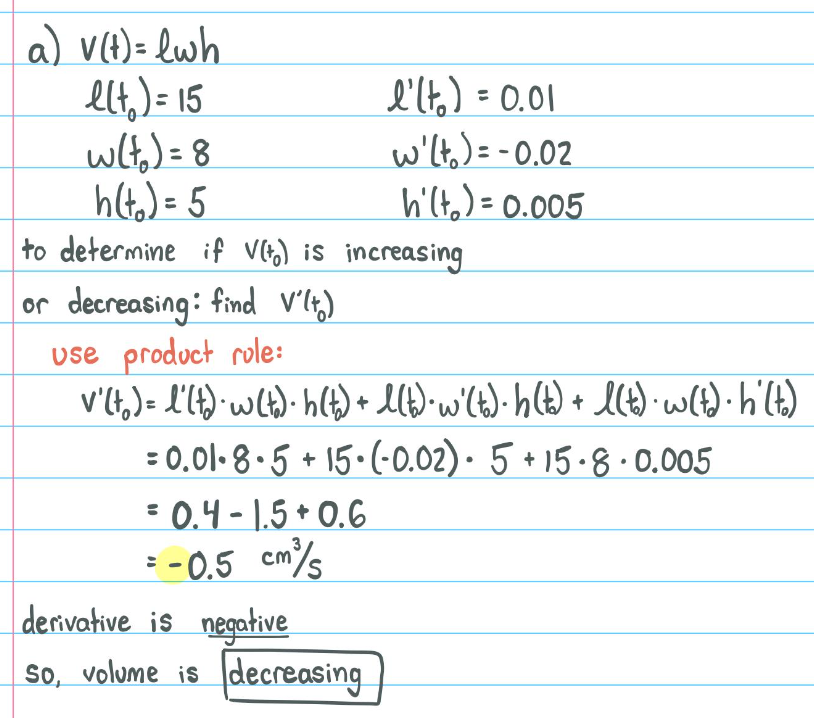
\includegraphics[width=\textwidth]{nice/p5.1a_isabella.png}
      Fun fact, if you think about it, you can see that the product rule and the multivariable chain rule are very related!
    \end{solution}
    \item Is the surface area increasing or decreasing at this moment?
    \begin{solution}
      We do the same analysis but with the function
      \[A(\ell,w,h)=2\ell w+2\ell h+2wh,\]
      which is the formula for surface area. Here is a solution by Sofia Tipple:

      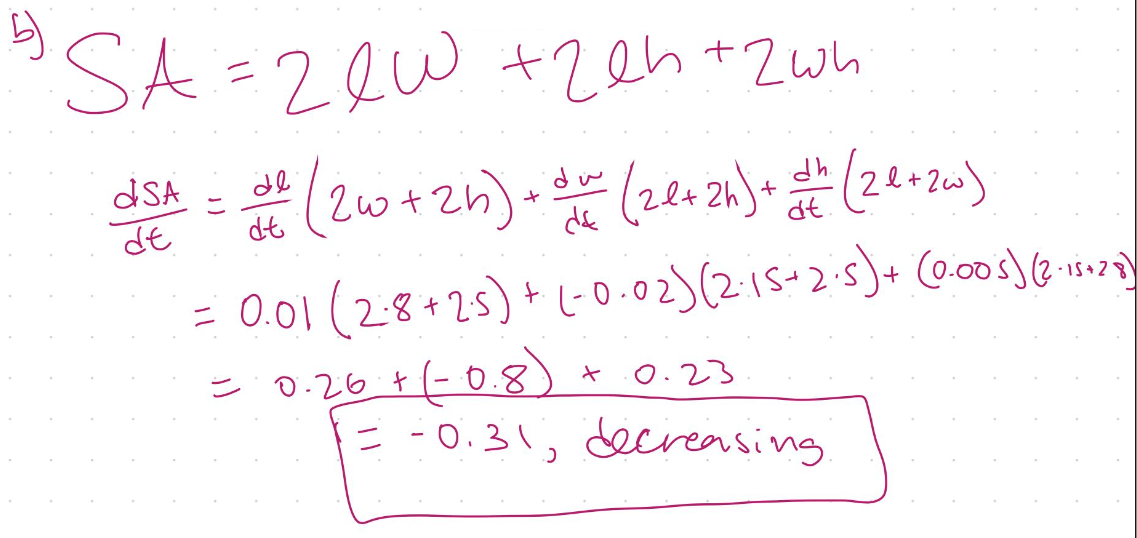
\includegraphics[width=\textwidth]{nice/p5.1b_sofia.png}
    \end{solution}
  \end{enumerate}
\end{problem}

\begin{problem}
  The directional derivative of $f(x,y)$ at $(1,2)$ along the unit direction parallel to $\bi+\bj$ is $2\sqrt2$. The directional derivative along the direction $-\bj$ is $-3$. Find the directional derivative of $f$ in the direction of $-\bi-2\bj$.
\end{problem}
\begin{solution}
  Remembering that $D_\bu f(P)$ is simply $\nabla f(P)\cdot \bu$, and that $\nabla f(P)=(f_x(P),f_y(P))$. Here we let $P$ stand for $(1,2)$ as is given in the problem. We see that we can solve for $f_x(P)$ and $f_y(P)$ using the given information, because they say:
  \begin{align*}
    D_\frac{\bi+\bj}{\sqrt2}f (P) &= 2\sqrt2\implies (f_x(P),f_y(P))\cdot \frac 1{\sqrt2}(\bi+\bj)=2\sqrt2,\\
    D_{-\bj}f(P) &= -3\implies (f_x(P),f_y(P))\cdot(-\bj)=-3.
  \end{align*}
  This transforms into:
  \begin{align*}
    \frac1{\sqrt2}f_x(P)+\frac1{\sqrt2}f_y(P) &= 2\sqrt2,\\
    -f_y(P) &= -3.
  \end{align*}
  So $f_y(P)=3$. If we plug this fact back into the first equation, we get $\frac 1{\sqrt2}f_x(P)+\frac1{\sqrt2}(3)=2\sqrt2$, which when solved yields $f_x(P)=1$. Finally,
  \[D_{\frac{-\bi-2\bj}{\sqrt5}}f(P)=(1,3)\cdot\frac{-\bi-2\bj}{\sqrt5}=-\frac7{\sqrt5}.\]
\end{solution}

\begin{problem}
  Consider the function $f(x,y)=x^2-y^3$. Let $P=\left(\frac12,1\right)$. Which direction $\bu$ will have the property that $D_\bu f\left(\frac12,1\right)=\sqrt{10}$?
\end{problem}
\begin{solution}
  We have $\nabla f(x,y)=(2x,-3y^2)$. And $\nabla f(\frac12,1)=(1,-3)$. We must solve the equation
  \[(1,-3)\cdot\bu=\sqrt{10}\]
  subject to $\|\bu\|=1$. To do this, let $\theta$ represent the angle between $\bu$ and $(1,-3)$, then we can express the dot product using the cosine angle formula:
  \begin{align*}
    \|(1,-3)\|\|\bu\|\cos\theta&=\sqrt{10}\\
    \iff \|(1,-3)\|\cos\theta &=\sqrt{10},\quad\text{because }\|\bu\|=1,\\
    \iff \sqrt{10}\cos\theta&=\sqrt{10}\\
    \iff\cos\theta&=1\\
    \iff \theta&=0.
  \end{align*}
  This last line says that $\bu$ is actually the unit vector pointing in the exact same direction as $(1,-3)$, which is $\frac1{\sqrt{10}}(1,-3)$.

  There are other solution methods possible. Here is a more algebraic solution by Hannah Roche:

  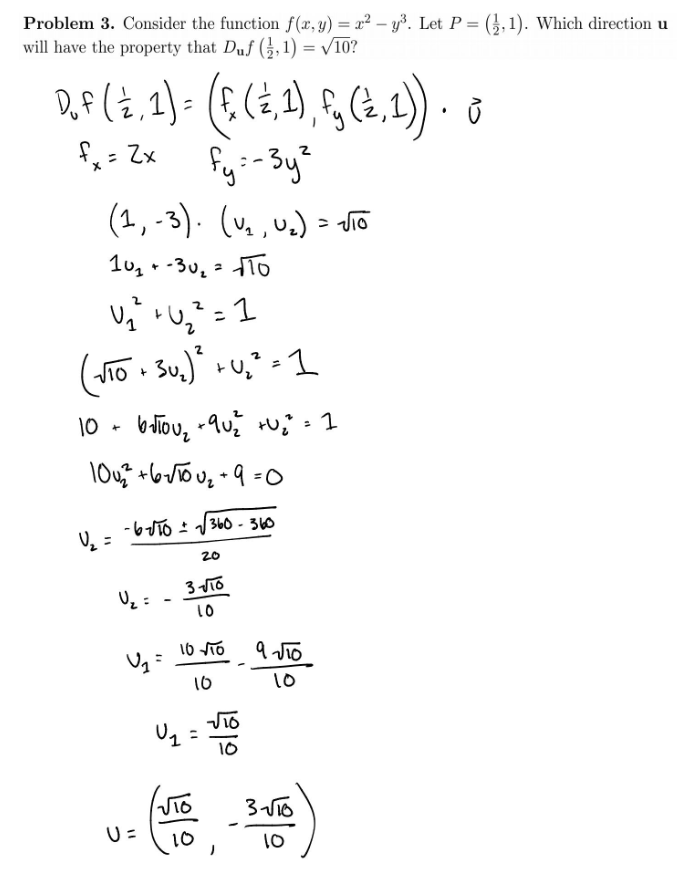
\includegraphics[width=\textwidth]{nice/p5.3_hannah.png}
\end{solution}

\begin{problem}
  Find the point on the surface $6x+y^2-z^2=3$ where the tangent plane is parallel to the plane $3x+y-2z=-5$.
\end{problem}
\begin{solution}
  The main idea that makes this problem tractable is to recall the theorem that the gradient of a function at a point is perpendicular to the level set of the function at that point. The key idea is that this holds in any number of dimensions, not just 2. (Indeed, see Theorem 1 on p.924 for the case of 3 variables.)

  Here, $6x+y^2-z^2=3$ is the level set of the function $f(x,y,z)=6x+y^2-z^2$ at 3. Hence, the tangent plane to this surface at any point $(x_0,y_0,z_0)$ (the point must be on the surface, of course) will have normal vector precisely equal to $\nabla f(x_0,y_0,z_0)$. For this function we calculate
  \[\nabla f(x_0,y_0,z_0)=(6,2y_0,-2z_0).\]
  The question asks for the point $(x_0,y_0,z_0)$ for which $(6,2y_0,-2z_0)$ is parallel to $(3,1,-2)$ (the normal to the plane $3x+y-2z=-5$). If we set up the equation
  \[(6,2y_0,-2z_0)=\lambda (3,1,-2),\]
  we see right away from the first coordinate that $\lambda=2$, after which we see that $y_0=1$ and $z_0=2$. Finally, $x_0$ must be such that $(x_0,y_0,z_0)$ satisfies the equation $6x+y^2-z^2=3$. Plugging in $y_0=1$ and $z_0=2$ into the equation $6x_0+y_0^2-z_0^2=3$ gives us that $x=1$. So the point is $(1,1,2)$.
\end{solution}

\begin{problem}
  Let $f(x,y)=xy-y^4$ and $P=(8,-2)$. Prove that there is no direction $\bu$ such that $D_\bu f(P)=50$.
\end{problem}
\begin{solution}
  Here I will show 3 solutions. First solution:

  We have
  \[\nabla f(8,-2)=(y,x-4y^3)\Big|_{(8,-2)}=(-2,40).\]
  So we need to prove there is no unit vector $\bu$ such that $(2,-40)\cdot\bu=50$.

  Recall that the Cauchy-Schwarz inequality says that for all vectors $\bv$ and $\bw$,
  \[|\bv\cdot \bw|\leq\|\bv\|\|\bw\|,\]
  (recall this just follows from the cosine angle formula for dot product along with the inequality $|\cos\theta|\leq 1$), which is equivalent to
  \[-\|\bv\|\|\bw\|\leq \bv\cdot \bw\leq \|\bv\|\|\bw\|.\]
  Here, let's use $\bv=(-2,40)$ and $\bw=\bu$. Keeping in mind that $\|\bu\|=1$, we see that
  \[-\sqrt{1604}\leq (2,-40)\cdot\bu\leq\sqrt{1604}.\]
  As $\sqrt{1604}\approx 40.05$ and is less than 50, we see there does not exist $\bu$ such that $(2,-40)\cdot\bu=50$.

  The second solution proceeds similarly to the first but achieves a crude upper bound of 42 by considering the system of equations:
  \begin{align*}
    -2u_1+40u_2 &= 50\\
    u_1^2+u_2^2 &= 1.
  \end{align*}
  The second equation implies $-1\leq u_1\leq 1$ and $-1\leq u_2\leq 1$, meaning that the value of $-2u_1+40u_2$ cannot exceed $-2(-1)+40(1)=42$. (Food for thought: The maximum achievable value is actually less than 42. Why?)

  The third solution takes the system of equations from the second solution and reduces it to a quadatic in one of the variables, then evaluates the discriminant of the quadratic to determine if it has solutions. A lot of you had this solution. I guess that my discussion of quadratic equations in class sparked this idea. Very cool! Example solution by Eesha Ampani:

  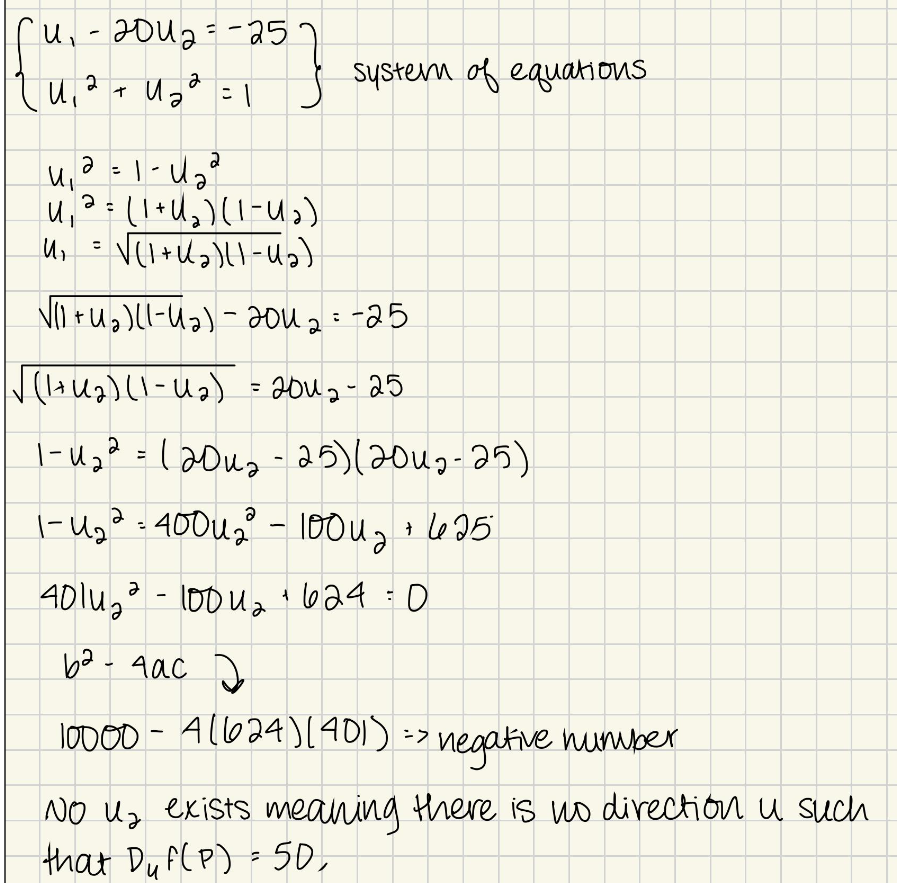
\includegraphics[width=\textwidth]{nice/p5.5_eesha.png}
\end{solution}

\begin{problem}
  How difficult was each problem? Rate each problem (and part) on a difficulty scale from 1 to 7, where 1 means ``super easy, barely an inconvenience!'' and 7 means ``hardest problem I've ever done.''
\end{problem}

\newpage

\section{Hints}
\begin{hint}[Hint for 2]
  Find $f_x(1,2)$ and $f_y(1,2)$ first. To check your answer, you should get $-7/\sqrt5$.
\end{hint}

\begin{hint}[Hint for 3]
  First, find the corresponding angle.
\end{hint}
